\section{Results}
\label{sec:results}

Table~\ref{tab:metrics} gives the metrics of the TF-IDF and logistic-regression detector at the threshold of Eq.~\eqref{eq:threshold}. Recall is 0.979 for the original and for the paraphrased e-mails: 95 of 97 phishing e-mails are detected in both versions. The realised false-positive rate is 0.49\% (11 of 2,231 legitimate test e-mails), below the target of 1\% and the guardrail of 2\%. The detector is deterministic, so the five seeds give identical values and the interval over seeds has zero width; the 95\% Wilson interval over e-mails is therefore shown instead.

\begin{table}[t]
\caption{Detector metrics at FPR$\,\le\,$1\% (97 phishing, 2,231 legitimate test e-mails).}
\label{tab:metrics}
\centering
\small
\begin{tabular}{@{}lcc@{}}
\toprule
Metric & Original & Paraphrased \\
\midrule
Recall & 0.979 & 0.979 \\
Recall, 95\% Wilson CI & [0.928, 0.994] & [0.928, 0.994] \\
Realised FPR & 0.0049 & 0.0049 \\
Precision & 0.896 & 0.896 \\
F1 & 0.936 & 0.936 \\
ROC-AUC & 0.9997 & 0.9996 \\
\bottomrule
\end{tabular}
\end{table}

For RQ1, the paired outcome of Eq.~\eqref{eq:discordant} is $b=0$ and $c=0$: no e-mail was lost and none was gained. The one-sided exact McNemar test gives $p=1.0$ (Holm-adjusted $p=1.0$), so $H_0$ is not rejected. The one-sided 95\% upper bound of the share of e-mails lost to paraphrasing is 3.0\%.

Paraphrasing did change the scores. The mean paired shift is $\delta=-0.53$ (95\% bootstrap CI $[-0.67,-0.39]$). Fig.~\ref{fig:margin} shows the score margin of every phishing e-mail, that is, its score minus the threshold. The median margin of the original e-mails is 4.27. Table~\ref{tab:model} compares the location-shift model of Eq.~\eqref{eq:shift} with the measurement. The ratio of the standard deviations (paraphrased to original) is 0.98. The break-even shift of Eq.~\eqref{eq:breakeven} for a loss of $d=2$ percentage points is $-1.10$. The model predicts a paraphrased recall of 0.992 against the measured 0.979, an absolute error of 1.2 percentage points.

\begin{figure}[t]
\centering
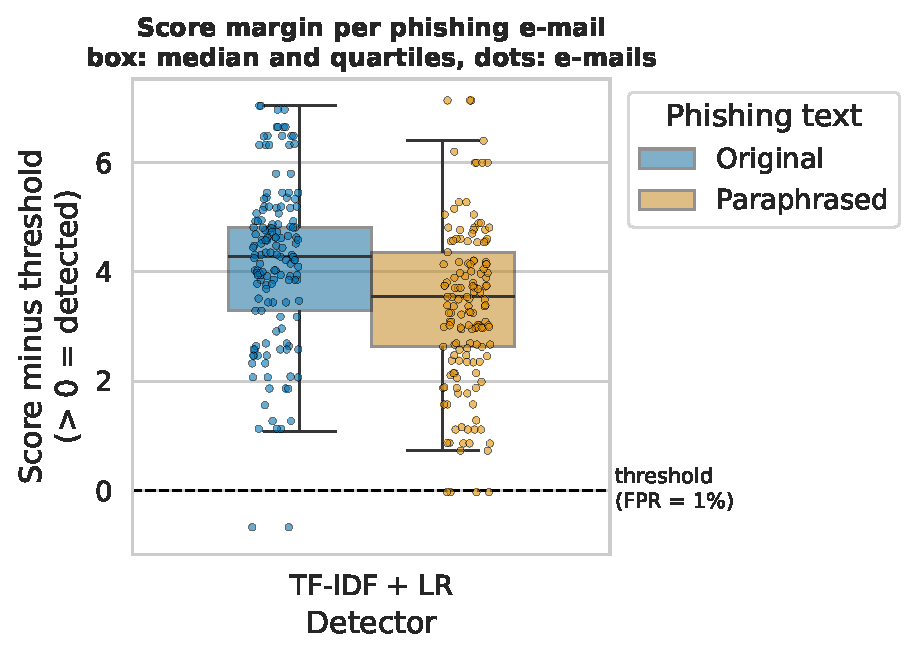
\includegraphics[width=\columnwidth]{figures/fig2_score_margin_distribution.pdf}
\caption{Score margin (score minus threshold) of the 97 phishing e-mails, original and paraphrased. Higher means farther above the threshold.}
\label{fig:margin}
\end{figure}

\begin{table}[t]
\caption{Location-shift model against measurement.}
\label{tab:model}
\centering
\small
\begin{tabular}{@{}lcc@{}}
\toprule
Quantity & Measured & Model \\
\midrule
Recall, original & 0.979 & 0.997 \\
Recall, paraphrased & 0.979 & 0.992 \\
Score shift $\delta$, 95\% CI & \multicolumn{2}{c}{$-0.53$ $[-0.67,-0.39]$} \\
Median margin, original & \multicolumn{2}{c}{4.27} \\
Break-even shift, $d=2$ p.p. & \multicolumn{2}{c}{$-1.10$} \\
\bottomrule
\end{tabular}
\end{table}
